\documentclass[11pt]{article}
\usepackage{amnat}
\usepackage{rotating}
\usepackage[english]{babel}
\usepackage[T1]{fontenc} % for Polish character
\usepackage{threeparttable} % for footnote below the table

% Tell latex how it can introduce linebreaks if necessary.
\hyphenation{Bar-thol-o-mew}

\begin{document}

%--------------------------------------------------
% Titlepage and Abstract
%--------------------------------------------------

% The first page of the manuscript file should be a title page that includes
% the title; a list of four to six keywords; and a list of all the elements of
% the manuscript that will appear in the expanded online edition (so reviewers
% will not miss essential elements). The title page should indicate whether the
% manuscript is an article, note, synthesis, natural history miscellany,
% comment, reply, or symposium (invited) article.

%Key words: Energy budget, body mass, temperature, thermoregulation (or thermodynamic), metabolic rate, foraging rate

\title{Net energy gain as a function of body mass and temperature}

% removed for anonymity during review
% LATER: restore, and add addresses
% \author{
%     Tanjona Ramiadantsoa \& Emma E.\ Goldberg
% }

\date{}

\maketitle

% \bigskip

% \noindent
% \textit{Manuscript elements}:
% Figures 1--5.
% Table 1.
% No color.
% Appendix:  Mathematical definitions,  derivations, and sensitivity analyses

% \bigskip

% \noindent
% \textit{Keywords}:
% thermal performance, body mass, temperature, warm-up, metabolic rate, foraging rate

% \bigskip

% \noindent
% \textit{Manuscript type}:
% Article.

% \vfill

%\noindent{\footnotesize Prepared using the suggested \LaTeX\ template for \textit{Am.~Nat.}}

% \newpage

% The second page should be the one-paragraph abstract, without citations, of
% less than 200 words for articles.

\linenumbers{}
\modulolinenumbers[2]

\section*{Modeling warm-up process} % (fold)
\label{sec:modeling_warm_up_process}
%
We make the following assumptions.
First, daily air temperature is simplified to a sine function,
\begin{equation} \label{eq:Ta}
	T_a(t) = \overline{T_a} + \nu \sin(\omega t),
\end{equation}
where $t$ is time of the day starting at sunrise, $\overline{T_a}$ is the average daily temperature, $\nu$ is the amplitude of the fluctuation, and $\omega = 2 \pi /24 h$ is the period.

Second, the operative temperature of an individual of mass $z$ is 
\begin{equation} \label{eq:Te}
	T_e(z,t) = T_a(t) + T_d(z),
\end{equation}
where $T_d(z)$ pools the effects of thermal environment (solar radiation, convection, conductance and so on) on the individual. 
There are exact formulas for calculating and also approximating $T_d$ \citep[e.g.,][]{Stevenson1985, Angilletta2009} but instead we use the following simplified (justified?) equation
\begin{equation} \label{eq:Td}
 	T_d(z) = T_d(z_0) + \delta_T \log_{10} \left(\frac{z}{z_0} \right).   
\end{equation} 
 The equation above states that for a 10-fold increase in body mass, the operative temperatue increases by $\delta_T$ degree Celsius.
 The smallest individual we consider here has mass $z_0$ with a maximum increase $T_d(z_0)$.
 The idea comes from \citet{Stevenson1985} which suggested that an 10-fold increase in body mass raises the maximum body temperature an individual can attain by $4.5 ^\circ \rm{C}$.
 We are making an implicit assumption here that the maximum body temperature and maximum operative temperature are equal (justified?).

 Third, the change in body temperature $T_b$ follows Newton's law of heating/cooling,
 \begin{equation} \label{eq:Tb0}
 	\frac{T_b(z,t)}{dt} = \frac{k_c(z)}{Q(z)} \left( T_b(z,t) - T_e(z,t)\right),
 \end{equation}
 where $k_c(z)$ is the heat transfer coefficient and $Q(z)$ is the heat capacitance of the individual.
The heat capacitance is simply mass times the specific heat capacity i.e., $Q(z) = z s$.
We simplify the heat transfer coefficient such that it is proportional to the surface area of the individual i.e. $k_c(z) = \alpha' z^{2/3}$.
By replacing $T_e(z,t)$ in \cref{eq:Tb0} by its expression in \cref{eq:Te}, and $T_a(t)$ and $T_d(t)$ by \cref{eq:Ta} and \cref{eq:Td}, respectively, we have
\begin{equation} \label{eq:Tb}
	\frac{T_b(z,t)}{dt} = \frac{\alpha}{z^{1/3}} \left[ T_b(z,t) - \nu \sin(\omega t) - f(z) \right],
\end{equation} 
where $\alpha = \alpha'/s$, and $f(z)$ is a time independent function $f(z) = \overline{T_a} + T_d(z_0) + \delta_T \log_{10} \left( \dfrac{z}{z_0} \right)$.
%
The advantage is that \cref{eq:Tb} has a closed form solution.
% section modeling_warm_up_process (end)


\section{Cost of warm-up} % (fold)
\label{sec:cost_of_warm_up}
In the preview version, we assumed that if $\tau_f$ is the total time to acquire a quantity of resource $R$, $\tau_f = R/g(z)$, then the actual foraging time is $\tau_f - \tau_w$. 
I suggest we assume a depletion rate that is independent of body size. 
If warm-up starts at time $t_0$ then the amount resource available decreases at a certain rate (whatever linear or exponential which can also be parameterized).
It might be a better way of envisioning competition. 
The motivation is to think about an elephant dung that is gradually depleted.

% section warm_up (end)







% \begin{abstract}
% \noindent
Empirical studies have reported that fitness first increases but eventually decreases as temperature increases, at least for ectotherms.
Although body mass is a key intrinsic factor that influences fitness, its role in shaping such hump-shaped thermal performance curves remains an open question.
In this work, we ask whether performance as a function of temperature broadens, shrinks, or shifts when body mass increases.
We build a model that integrates ecological (foraging), physiological (metabolism), and thermodynamic (warm-up) processes and asks how their interplay shapes the daily net energy gain, which we use as a proxy for performance.
We found that there is no single expected relationship of how the thermal performance curve changes with body mass, but foraging shapes its upper limit and warm-up ability determines its lower limit.
More generally, the model aims to fuel feedback between empirical and theoretical work by identifying important parameters and relationships amenable to empirical investigations, and by proposing how the three types of processes may influence species' geographic distribution.

% \end{abstract}

% \newpage

% %--------------------------------------------------
% % Content: see other .tex files
% %--------------------------------------------------

% \input{./1_{}Introduction.tex}
% \input{./2_Materia{}l_and_methods.tex}
% \section*{Results}
The results are partitioned into 3 parts.
Many things go into performance. We  single out the effects here.
 Ask, when can performance peak at intermediate body size.

- Physiological and ecological processes.
When resource or time is limiting.

Fig 1 shows how net gain changes as function of body size

 Case 1: when resources are low, the gain cannot compensate for large and thus net gain decreases with body size. 
 This effect vanishes as resource increases, net energy gain increases as function of body mass.
 What it is interesting here is that exponent of foraging rate, or metabolism, and metabolic scope interferes only quantitatively. 
 
 Case 2: we now look at the role of temperature.
 Temperature increases the metabolic cost.
 Foraging is constant here but we vary the cost being active ($b_2 = 1.25, a_2 = 40$).
 Even if resources are unlimited.
 As temperature increases, it becomes more costly for large given that $b_3$ is low. 
 The ratio plays a role here.
 As a contrast, when b3 is high, only large can persist. 

 It is worth to mention that foraging time differs here and this for low b3, it takes longer for large to get 50 times the resources and thus even higher active metabolic rate   
 
 Fig 2 shows when time is limiting
 In the same scenario as above, large is always advantageous when b3 is high enough.
 When b3 is low the same hump pattern occurs.
This only happens at specific situation.
First, net energy can should increases and then decrease after certain threshold (thus looking at the derivatives)
Second, net energy should also be positive.
These conditions are fulfilled when: 

 There are two things: the $b_3$ as we have seen before but also, resource quality matters.
 Sound too restrictive. 
 

We explored the influences of two internal parameters: $b_3$ (\cref{eq:eg}) which scales the effect of body size on resource allocation and conductance $K_1$ and $K_2$ which defines the passive loss of heat during warm-up, convection, and two environmental variables: environmental temperature $T_e$ and the amount of resource available $R$.

Our main goal is to understand the role of different processes in shaping the energy budget of a species given its body mass.

% E: Good strategy to give basics of model behavior first, and then put it together for the more complicated niche questions!

\subsection*{Role of foraging and cost of metabolism}
We look at the cases that can limit the amount of resources that an individual can acquire.
The first case is when the amount of resource available is limited (\cref{fig1}).
When there is not enough resource, the high energetic demand of large individual due to higher metabolic rate cannot be compensated.
As a consequence, as net energy gain decreases as function of body size (\cref{fig1}ab).
When resources are not limiting, net energy gain increases with body size.
More importantly, the foraging exponent $b_3$ only changes the pattern qualititatively.

The situation may be different when temperature is varied.
By increasing the metabolic scope (high cost of activity), large individual shows two contrasting responses.
When foraging exponent is low ($b_3 = 0.5$ ), performance is again maximized at intermediate value even if resources are not limiting (\cref{fig1}d vs. \cref{fig1}e).
Increasing temperature puts more pressure on large individuals as the metabolic cost is higher.
When foraging exponent is high $b_3 = 1.25$, only large individual can persist (\cref{fig1}f).

The second case is when the time available for foraging is limited (\cref{fig2}).
In general, net energy gain increases as function of body size.
However, like in the previous case, when $b_3$ is low, maximum net energy gain is attained at intermediate body size (dashed line, \cref{fig2}a). 
The analytical result shows that net energy gain only peaks when two conditions  are met.
First, $b_3 < b_1 = b_2$ (the equality is by assumption and to reduce the number of free parameter).
% E: so really, the condition is that b_3 is the smallest? 
% T: yes
Second, resource quality $\rho$ is within a certain range represented by shades in \cref{fig2}a.
\cref{fig2}b shows for two different temperatures (red = warm, blue = cold) the required values of the resource quality $\rho$ so that net energy gain peaks at intermediate value of body mass.
\cref{fig2}c shows how net energy gain changes as function of body mass for the resource quality shown in \cref{fig2}b.
These conditions are quite restrictive and looks unlikely in real system.
% E: This is a great example of why it was worth constructing a math model, rather than just intuitive arguments!

In a more technical term, the range of the $\rho$ allowing intermediate optimal body mass is 
\begin{equation}\label{C1}
	\widetilde{E_n} < \rho < \widetilde{dE_n}.
\end{equation}
where,
\begin{flalign*}
\widetilde{E_n} &= \theta_1 + \theta_2, \\
\widetilde{dE_n} &= \frac{b_2}{b_3} \theta_1  +  \frac{b_1}{b_3} \theta_2.
\end{flalign*}
and $$\theta_1 = \frac{a_2}{a_3}  z^{b_2 - b_3}  e^{-E/[k (max(T_w(z_{th}),T_e(t))+ 273.15)]}$$ and $$\theta_2 =  \frac{a_1}{a_3} z^{b_1- b_3}  e^{-E/[k (T_e(t)+ 273.15)]} (\frac{24}{t_f} -1).$$

The difference between  $\widetilde{E_n}$ and  $\widetilde{d E_n}$ is that in  $\widetilde{dE_n}$, each term of  $\widetilde{E_n}$   is weighted by $\frac{b_2}{b_3}$ and $\frac{b_1}{b_3}$.
Thus, a necessary condition for optimal mass to be intermediate (\cref{C1}) is that the weights are larger than 1 i.e.  $b_3 < b_1$ ($b_2 \geq b_1$ is always true). 
As temperature increases, the term with the product $\frac{b_1}{b_3}$ becomes larger thus increasing the range of values where \cref{C1} is true (\cref{fig2}a).

Note  that the bandwidth is broader in warm than in cold environment.
This is because in warm environment , the $\theta$s are larger arithmetically and not geometrically.
It is easier to use example. 
For simplicity, if $\theta_1 = \theta_2 = 1 (10)$ small (or large) and $b_1 =b_2 = 0.75, b_3 = 0.5$.
For small, the range is $\theta_1 + \theta_2 = 2 < \rho <  0.75/ 0.5 \theta_1 +  0.75/0.5 \theta_2 = 3.$  
For large, the range is $\theta_1 + \theta_2 = 20 < \rho <  0.75/ 0.5 \theta_1 +  0.75/0.5 \theta_2 =  30.$  


\subsection*{Role of warm-up.}
\subsubsection*{Minimum conditions}
Successful warm-up is a necessary condition before foraging. 
Under perfect conditions where solar radiation is not limiting and forced convection from wind is absent , any individual can absorb use that energy to warm-up.
We explore here cases where solar radiation is limiting and wind increasing convection between the surface of the individual and the external environment.

Three different ways the minimum temperature required to complete warm-up vary as a function of body mass (\cref{fig3}).
First, the minimum temperature for warm-up increases with body mass because small individual absorbs more heat--higher surface area-to-body ratio (\cref{fig3}a).
This pattern only occurs when the individual relies only solar radiation to warm-up (ectotherm) and there is only free convection (no wind).
Second, the minimum temperature for warm-up is lowest at intermediate body size (\cref{fig3}b). 
This happens because there is now more convection due to wind. 
Small individuals are  penalized as convection increases (see \cref{eq:dTr2}).
Third, minimum temperature decreases with body size (\cref{fig3}c).
It occurs when individuals are capable of producing heat endogenously (endotherm).
In this case, the role of surface area-to-body ratio is reversed as the heat generated in the thorax dissipates less with large individuals.
% E: I repeat my comment above: This is a great example of why it was worth constructing a math model, rather than just intuitive arguments!

\subsubsection*{Duration of warm-up.}
Another aspect of warm-up is the time it takes to complete it.
As expected, duration of warm-up decreases as this intensity of solar radiation increases (it peaks at noon) (\cref{fig4}).
The decrease is not linear, warm-up time decreases abruptly and then level off few hours after sunrise (\cref{fig4}a).
For endothermic individual, the same pattern occurs although it is less abrupt compared to ectothermic individuals (\cref{fig4}b) .
For ecothermic individuals, the duration of warm-up increases with body mass (\cref{fig4}a).
For endothermic, it is not necessarily true because the smallest individual can lose too much of the heat it generates to the environment via conductance (\cref{fig4}b).

Conductance between the thorax and the rest-of-the-body plays an important role for the warm-up process and, as expected, has opposing roles for ecotherm and endotherm.
For endotherm, \cref{fig4}c shows how different values for the conductance are favored at different parts of the day.
If warm-up is initiated early in the day where solar radiation is weak, low conductance is better (thick line \cref{fig4}c).
As the intensity of solar radiation increases, it becomes a dominant source of energy and transferring that energy to the thorax is better achieved with high conductance (dashed line \cref{fig4}c).

\subsection*{Niche as a sum of physiological and behavioral processes.}
Now we integrate those components together to see how they shape the net energy gain as function of temperature. 
We also include performance when daily temperature changes. 
In that case and for simplicity, we assume that temperature increases linearly from sunrise to mid-afternoon and then decreases again (see appendix). 
There is no temperature at the previous and next sunrise.

\cref{fig5}a shows a default scenario with intermediate resource abundance.
For a range of daily temperature, net energy gain is highest at intermediate body size, large is not optimal for the same reason as in \cref{fig1}.
As resource abundance decreases, net energy gain decreases for larger individuals (solid lines \cref{fig5}b).
This makes small individual (relatively) more competitive and actually perform better at high temperature.
Also note that the upper limit of the `niche' is contracted to lower temperature (\cref{fig5}b), simply because the amount of resource available does not compensate the high energetic cost.

When we integrate warm-up processes, which is important when temperature is cold, large individual is also more affected.
Because it takes too much time to warm-up (\cref{fig4}bc) whether one is endothermic or ectothermic.
We assumed here that time spend during warm-up is subtracted in the total time available for foraging.
In short, warm-up contracts the lower part part of the niche.
Supplementary material contains more detailed results where warm-up cannot be completed so that the lower limit will be dictated by the patterns in \cref{fig3}.
...
% E: discuss endo vs ecto?

Finally, we look at variation in daily temperature.
Instead of having constant daily temperature, we assumed that increases throughout the day.
This increases in temperature further affects the largest individual (thick line in\cref{fig5}d).
The first reason is depicted in \cref{fig1}def where temperature increases disproportionately increases the energetic demand of large individuals even if resources are unlimited.
The decline of large individual will be unavoidable when resources are limiting (\cref{fig1}ab and \cref{fig5}d).




% \section*{Discussion}
Know the fundamental niche, reaction norm, proxy for fitness, performance curve.
Many models
Niche Mapper
Buckley model
Brown

General model
Complexity for parameterization

Body size and temperature

Endotherm and nocturnal.


Behavior: Warm-up, timing of dial and seasonal activity (supported by Kearney)
Limited or increased foraging time. 

Importance of foraging.
Resource availabilty. 
Kearney vegetation cover.

Non linearity in evolutionary model

Influence of fluctuating temperature

Missing:
humidity
conversion to offspring
mortality



}
% %\input{./Appendix_warm-up_derivation.tex }

%--------------------------------------------------
% \section*{Acknowledgements}
%--------------------------------------------------
% LATER: include in pdf.  Removed for anonymity now.

%--------------------------------------------------
% References
%--------------------------------------------------

% \clearpage

\setstretch{1.5}
\bibliography{refs_energy_budget}
\bibliographystyle{amnat}
% LATER: paste .bbl file here (actually, see latex instructions accessible from upload page)

%--------------------------------------------------
% Tables, Figures, Captions
%--------------------------------------------------

% \clearpage
% % E: Some suggestions for fitting this on one page: prune words from Definition, smaller font, references as footnotes

\begin{sidewaystable}
\caption{Values and ranges of parameters used }
\begin{tabular}{l l l l l}
\hline
Notation& Definition & Value or range & Unit & References \\
\hline
&\textbf{Intrinsic body size scaling} & & &  \\
$a_1$ & Coefficient for resting metabolic rate  & $\propto 1$  & $\rm{J \, s}^{-1}$ & \citet{Heinrich1975} \\
$b_1$ & Exponent for resting metabolic rate  & 0.75 &  & \citet{Kleiber1947,Peters1986} \\
      &                                      &      &  & \citet{Gillooly2001} \\
$a_2$ & Coefficient for active metabolic rate  & 10-30 $ \times a_1$ & $\rm{J \, s}^{-1}$ &  \citet{Bartholomew1981}; \\
      &                                        &                     &                    &  \citet{Niitepold2010} \\
$b_2$ & Exponent for active metabolic rate  & 0.75-1.25 & &  \citet{Heinrich1975} \\
$a_3$ & Coefficient for foraging rate  & 1 & $\rm{g \, s}^{-1}$  & \\
$b_3$ & Exponent  for foraging rate  & 0.5-1.25 &  &  \citet{Pawar2012, Nervo2014}; \\
      &                              &          &  &  \citet{Maino2015} \\
$c_0$ & Intersect for minimum temperature for activity & 28 & $^{\circ}\rm{C}$  & \citep{Bartholomew1977a}* \\
$c_1$ & Slope for minimum temperature for activity & 0.75 &  $\rm{g \,  ^{\circ}C^{-1}}$ &  \citep{Bartholomew1977a}* \\
%\hline
& \textbf{Physical and thermodynamic constants} & & &  \\
$\delta $ & mass density & $0.15 \times 10^6$  & $\rm{g \, m}^{-3}$  & personal data\\
$a_w$& Constant for frequency of contraction & 0.25 & $\rm{s}^{-1}$   & \citet{Bartholomew1977b}*\\
s & specific heat capacity & 3.3472 & $\rm{J \, g}^{-1}\,\rm{C}^{-1}$ & \citet{Heinrich1975} \\
e & Energy per contraction & 0.04184 & $\rm{J \, g}^{-1}$ &\citet{Kammer1974} \\
$K_1$& Conductance between the thorax and the rest-of-the-body & 0.05 $c_p$ & $\rm{J \,s}^{-1} \, \rm{m}^{-2} \, ^{\circ}\rm{C}$  & \citet{Campbell2012} \\
$K_2$& Constant controlling convection & 1   & $\rm{J \,s}^{-1} \, \rm{m}^{-2} \, ^{\circ}\rm{C}$  & \citet{Campbell2012} \\
%\hline
& \textbf{Extrinsic constants} & & &  \\
$c_p$ & molar specific heat of air  & 29.3 &  $\rm{J \, mol}^ {-1} \, \rm{C}^ {-1}$ & \citet{Campbell2012} \\
u &  wind speed & 0.1 & $\rm{m \, s}^{-1}$ & \\
$\sigma$ & Stefan-Boltzman constant & $5.67 \times 10^{-8}$ &  $\rm{J \, m}^{-2} \rm{s}^{-1} \rm{K}^{-4}  $  &  \\
$\varepsilon$& Emissivity of gray body & 0.93& & \citep{Campbell2012} \\
$\rho$ &Energy density per gram of resource & 13-100 &  $\rm{J \, g}^{-1}$  &  \\  %  Energy density per gram  dry dung (40-80\%) of total weight, \citet{Nibaruta1980} \citet{Gittings1998}
$r_3$  & Scale factor for the quantity of solar radiation absorbed & 0.5 &  &  \\
\hline
\label{table:table1}
\end{tabular}
\raggedright{*means that the value is approximated.}
\end{sidewaystable}


% \clearpage
% \nolinenumbers % applies to the figures
% \section*{Figure captions}
\begin{figure}[H]
\begin{center}
%\scalebox{1.5}{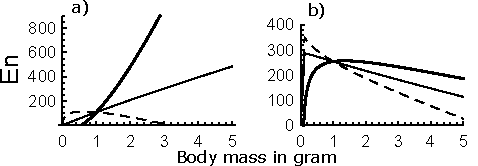
\includegraphics{Fig1}}
\caption{
	A caricature of how the exponent influences the concavity (convexity) of the power in the power law relationship.
	The black and gray lines represent foraging and active metabolic rates.
	The exponent of the metabolic rate is a bit lower to visualize to assure that the gain is more than the cost most of the time.
}
\label{fig1}
\end{center}
\end{figure}
\vspace{-1.5cm}
%
\begin{figure}[H]
\begin{center}
%\scalebox{1.5}{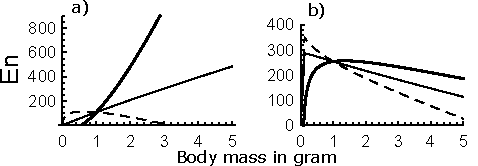
\includegraphics{Fig1}}
\caption{
	No warm-up and resource is limiting.
	Daily net energy gain  $E_n$ as function body mass $z$ for different value of foraging exponent $b_3 = 0.5, 0.8, 1.25$, dashed, thin, thick lines respectively.
	The upper panels depict different resource availabilities at $15 ^{\circ} \rm{C}$. 
	Low resource = 2.5, intermediate resource= 20, unlimited resource means an individual can collect 50 times its body mass, $b_2 = 0.75, a_2 = 20 a_1$. 
	The lower panels depict the influence of temperature when resources are unlimited and high active metabolic rate $a_2 = 40 a_1, b_2  = 1.25$.
	Low, mild, and high temperature = $5, 15, 25^{\circ} \rm{C}$.
	Fixed parameter values: $b_1 = 0.75, \rho = 16$.
}
\label{fig2}
\end{center}
\end{figure}
\vspace{-1.5cm}
%
\begin{figure}[H]
\begin{center}
%\scalebox{1.5}{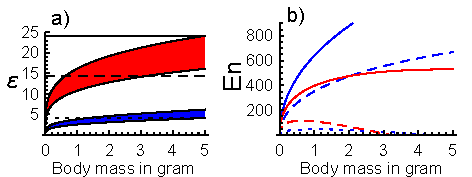
\includegraphics{Fig2}}
\caption{
	No warm-up and foraging time is limited to 0.5 hour.
	a) Daily net energy gain  $E_n$ as function body mass $z$ for different value of foraging exponent $b_3 = 0.5, 0.8, 1.25$, dashed,think, thick lines respectively  at $15 ^{\circ} \rm{C}$.
	b) $E_n$ is maximized at intermediate value of $z$  when shaded regions and resource quality $\rho$ intersect (i.e., \cref{C1} is satisfied).
	Warm ($35^{\circ} \rm{C}$) and cold (15$^{\circ} \rm{C}$) environmental temperatures are denoted by red and cyan, respectively.
	The upper (lower) limit of the shade region is $\widetilde{dE_n}$ ($\widetilde{E_n}$).  
	c) Various shapes of $E_n$ based on b).
	In b) and c), $\rho = 13, 60, 100$ dashed, thin, and thick, respectively.
	Fixed parameter values: $b_1 = b_2 = 0.75, a_2 = 5 a_1, $.
}
\label{fig3}
\end{center}
\end{figure}
\vspace{-1.5cm}
%
\begin{figure}[H]
\begin{center}
%\scalebox{1.5}{\includegraphics{Fig3}}
\caption{
	Lowest temperature required for the completion of warm-up as a function of body mass.
	The individual is given a maximum of 6 hours to complete warm-up.
	The thorax is half of the total body mass.
	To focus on the effect of solar radiation, daily temperature is constant.
	Solar radiation increases linearly from 0 to 0.25 of the maximum value $S_0$ during a period of 6 hours. 
	a) conductance is low (0.1 $\times$ the default value).
	b) conductance is default, wind speed  = 0.1m/s.
	c) For endotherm with free convection $a_w = 1.25$. 
	Fixed parameter values: default conductance $K_1 = 0.05 c_p, r_3 = 0.5$.
	Remaining parameters are in table 1.
}% Add parameter values later
\label{fig4}
\end{center}
\end{figure}
\vspace{-1.5cm}
%
\begin{figure}[H]
\begin{center}
%\scalebox{1.5}{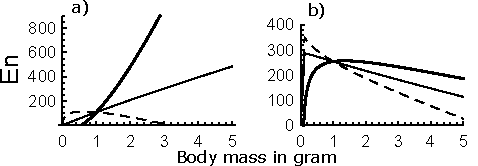
\includegraphics{Fig1}}
\caption{
	Duration of warm-up as a function of the timing of warm-up.
	Daily temperature varies from $15^{\circ}\rm{C}$ at sunrise and peaks at $30^{\circ}\rm{C}$ in the middle of the afternoon.
	Solar radiation is equivalent to what would happen at 30 degree latitude during to equinox clear sky.
	a) thickest, thick, thin, and dashed lines denote  $z = 10, 1, 0.1, 0.01$,  respectively.
	b)  Duration of warm-up with different conductance. Body size $z = 1$ , $a_w = 1.25$
	Default value for $K_1$ and $K_2$ .	
}% Add parameter values later
\label{fig5}
\end{center}
\end{figure}
\vspace{-1.5cm}
%%
\begin{figure}[H]
\begin{center}
%\scalebox{1.5}{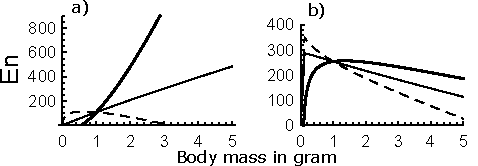
\includegraphics{Fig1}}
\caption{
	Shape of the fundamental niche as a function of temperature.
	a) As a function of when warm-up starts ($t_f = 1$ hour, early = sunrise, mid = sunrise+ 2 hr, late = sunrise + 4 hr, body size $z = 2$). 
	b) As a function of the exponent of $b_3$ ($t_f = 1$, large (black) = 2, small (gray) = 0.5).
	c)  As a function of resource availability. 
	Thick line = high resource (30), thin line = low resource (15).
	Thick and thin gray lines overlap because the small is not affected by resource loss. 
	  ($b_3 = b_2 = b_1 = 0.75$).
	Other parameters: $ b_2 = b_1  = 0.75,  a_2 = 10 a_1, a_w = 1.25$, and  $\rho = 30$.
}% Add non trivial units later
\label{fig6}
\end{center}
\end{figure}
%
%\begin{figure}[H]
%\begin{center}
%%\scalebox{1.5}{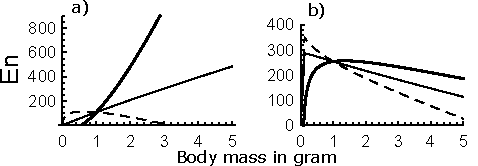
\includegraphics{Fig1}}
%\caption{
%	Shape of the fundamental niche as a function of temperature.
%	Except in d),  temperature is constant during the day.
%	a) The simplest case without warm-up, high resource availability (30 gram).
%	b) Halving resource availability and without warm-up.
%	c) Adding warm-up and  restoring resource availability to high, there is a penalty for long warm-up time as it reduces total foraging time, no change in temperature.
%	d) A complete  scenario with warm-up and variable temperature that increases from 15 to $30^{\circ} \rm{C}$ from sunrise to mid-afternoon.
%	Other parameters: $b_3 = 1, b_2 = b_1  = 0.75,  a_2 = 10 a_1, a_w = 1.25$, and  $\rho = 20$.
%}% Add non trivial units later
%\label{fig6}
%\end{center}
%\end{figure}
%

\end{document}

Future direction notes:

focus on the fix resource
make a simple model for warm-up

Optimum, foraging


Warm-up focused review.
What they think about the other components? 
Make warm-up more detailed or simpler
Body shape...
Don't mention 50 times not as main assumption...which result matter

Find analytical results for warm-up and optimum...

x, y axis: (body mass, net energy gain), (temperature, net energy gain), (resource quantity and quality, optimum mass ), (temperature, optimum mass)

Check if the result is the same...optimum after...

